\chapter{Probabilités}

\section{Vocabulaire et fondamentaux}

\begin{definition}
Une \textbf{expérience aléatoire} est une expérience dont les issues sont connues sans que l'on puisse prédire laquelle se produira. 
L'ensemble de toutes les issues possibles est appelé l'\textbf{univers}, noté $\Omega$.
\end{definition}

\begin{definition}
Un \textbf{événement} est un sous-ensemble de $\Omega$. 
\begin{itemize}
    \item Un événement contenant une seule issue est un \textbf{événement élémentaire}.
    \item L'ensemble vide $\varnothing$ est l'\textbf{événement impossible}.
    \item L'ensemble $\Omega$ est l'\textbf{événement certain}.
\end{itemize}
\end{definition}

\begin{exemple}
On lance un dé à 6 faces. $\Omega = \{1, 2, 3, 4, 5, 6\}$.
L'événement $A$: "obtenir un chiffre supérieur ou égal à 5" est $A = \{5, 6\}$.
\end{exemple}

\section{Loi de probabilité et équiprobabilité}

\begin{definition}
Définir une \textbf{loi de probabilité} sur $\Omega = \{x_1, x_2, \dots, x_n\}$, c'est associer à chaque issue $x_i$ un nombre $p_i$ tel que :
\begin{enumerate}
    \item Pour tout $i$, $0 \le p_i \le 1$.
    \item $\sum_{i=1}^{n} p_i = p_1 + p_2 + \dots + p_n = 1$.
\end{enumerate}
\end{definition}

\begin{propriete}
La probabilité d'un événement $A$, notée $P(A)$, est la somme des probabilités des issues qui le composent.
\end{propriete}

\begin{propriete}[Équiprobabilité]
Si toutes les issues ont la même probabilité de se réaliser, on dit qu'il y a \textbf{équiprobabilité}. Alors :
\[ P(A) = \frac{\text{Nombre d'issues de } A}{\text{Nombre d'issues de } \Omega} = \frac{\text{card}(A)}{\text{card}(\Omega)} \]
\end{propriete}

\begin{remarque}
Dans les exercices, les expressions "dé équilibré", "pièce non truquée" ou "tirage au hasard" indiquent une situation d'équiprobabilité.
\end{remarque}

\section{Opérations sur les événements}

\begin{definition}
Soient $A$ et $B$ deux événements.
\begin{itemize}
    \item L'événement \textbf{contraire} de $A$, noté $\bar{A}$, est l'ensemble des issues de $\Omega$ qui ne sont pas dans $A$.
    \item L'événement \textbf{intersection} $A \cap B$ est constitué des issues appartenant à la fois à $A$ \textbf{et} à $B$.
    \item L'événement \textbf{réunion} $A \cup B$ est constitué des issues appartenant à $A$ \textbf{ou} à $B$ (au moins l'un des deux).
\end{itemize}
\end{definition}

\begin{propriete}
Pour tous événements $A$ et $B$ :
\begin{enumerate}
    \item $P(\bar{A}) = 1 - P(A)$
    \item $P(A \cup B) = P(A) + P(B) - P(A \cap B)$
\end{enumerate}
\end{propriete}

\begin{definition}
Deux événements $A$ et $B$ sont dits \textbf{incompatibles} si $A \cap B = \varnothing$. Dans ce cas, $P(A \cup B) = P(A) + P(B)$.
\end{definition}

\section{Représentations graphiques}

\subsection{Diagrammes de Venn}
Les diagrammes de Venn permettent de visualiser les ensembles.

% Illustration TikZ : Diagramme de Venn
\begin{center}
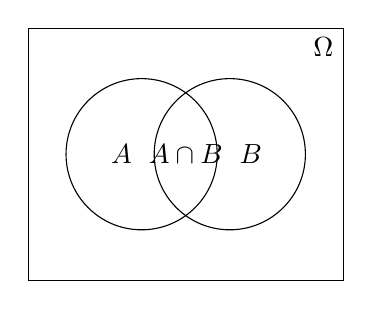
\begin{tikzpicture}[scale=0.8]
    \draw (0,0) rectangle (5,4) node[below left] {$\Omega$};
    \draw (1.8,2) circle (1.2) node[left] {$A$};
    \draw (3.2,2) circle (1.2) node[right] {$B$};
    \node at (2.5,2) {$A \cap B$};
\end{tikzpicture}
\end{center}

\subsection{Tableaux à double entrée}
Indispensables pour les expériences à deux critères (ex: une population avec genre et fumeur/non-fumeur).

\subsection{Arbres de dénombrement}
Utiles pour les expériences répétées ou à étapes successives.

% Illustration TikZ : Arbre simple
\begin{center}
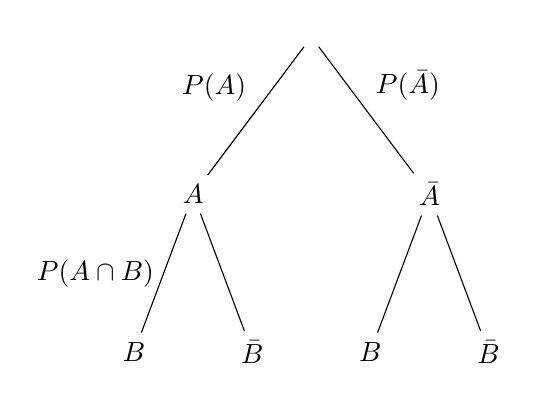
\begin{tikzpicture}[level distance=2cm,
  level 1/.style={sibling distance=3cm},
  level 2/.style={sibling distance=1.5cm}]
  \node {}
    child {node {$A$}
      child {node {$B$} edge from parent node[left] {$P(A \cap B)$}}
      child {node {$\bar{B}$}}
      edge from parent node[above left] {$P(A)$}
    }
    child {node {$\bar{A}$}
      child {node {$B$}}
      child {node {$\bar{B}$}}
      edge from parent node[above right] {$P(\bar{A})$}
    };
\end{tikzpicture}
\end{center}

\end{document}
